
\section{First approach}
Our first approach to design the product was to develop:

\begin{itemize}
\item A java 'Social' library that abstracted many common concepts found in different
social networks (Facebook, Twitter, LinkedIn..) like User, Post, Image and so on,
in order to give the developers the possibility to use and extend these concepts seamlessly
between different social networks. It would also handle the connection to the social networks,
to allow the developer to write full-fledged social 'multi-network' clients.

\item A java 'Communication' library to connect, using different interfaces, to the Arduino devices
in order to send the data fetched from the social networks. It would also provide a mechanism to manage
Arduino's firmware, to allow the device to support different hardware configurations.

\item A prototype showcasing the functionalities of the two libraries.
\end{itemize}

After the second meeting with the customer we decided to revise this plan, as this was not what
our customer really had in mind and also a bit ambitious. Some of the code and documentation we produced
earlier could be re-used, but some could not.

See appendix~\ref{app:firstdraftarchi} for more.

\newpage
\section{Revised approach}
The biggest difference in the new approach is that while the Social library will still provide
abstractions for concepts common found in social networks, it will now focus rather than handling
the connection to the social networks, on estabilishing a communication interface (using Android's Intent mechanism)
between Social applications and the Android-Arduino applications to allow them to request and forward 'social' data.

\begin{figure}[h!]
\centering 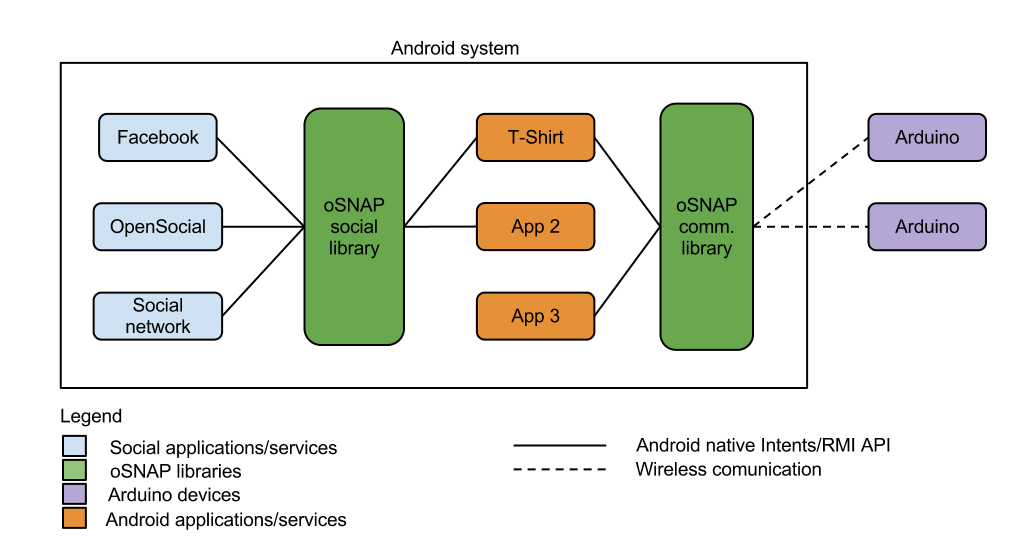
\includegraphics[scale=0.35]{img/architecture-toplevel.png}
\caption{Revised system architecture}
\label{fig:architecture-toplevel}
\end{figure}

\newpage

\subsection{First system design}
Our first system design was based on the scenario where the user would download the t-shirt
and the social applications, browse for some content from within the social application
and actively send it to the t-shirt application pressing a 'share' button.
This scenario is represented in figure \ref{fig:use-case1}

\begin{figure}[h!]
\centering 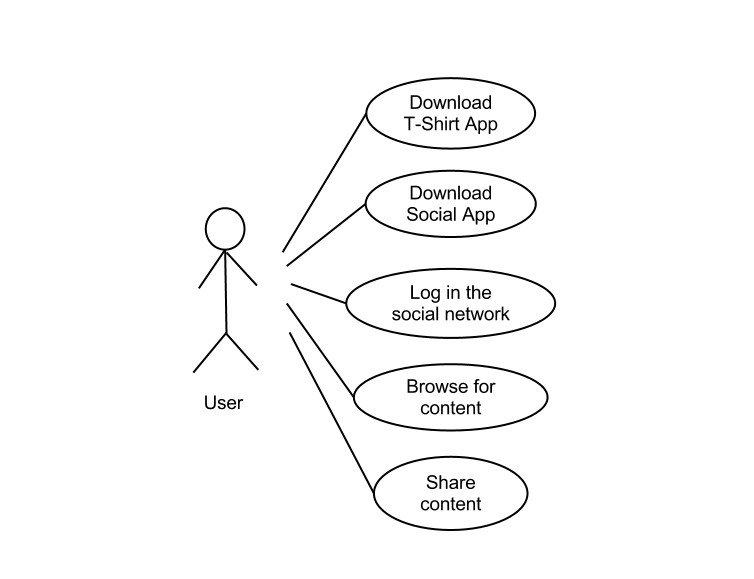
\includegraphics[scale=0.35]{img/architecture-usecase1.png}
\caption{Use case for the first design}
\label{fig:use-case1}
\end{figure}

Different sample applications following this design were developed and showed to the
customer for feedback, and this helped us realize at some point that this design wouldn't fit
the customer ideas for the final product.

\begin{figure}[h!]
\centering 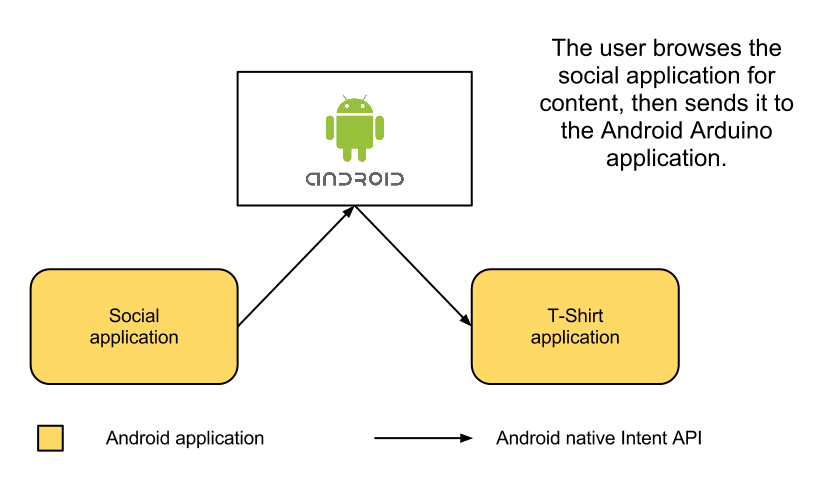
\includegraphics[scale=0.35]{img/architecture-resp.png}
\caption{}
\label{fig:resp}
\end{figure}

\subsection{Second system design}
Showing the customer various simple prototype applications in order to receive feedback we would use
to proceed with the system design, we understood that our first design was not really fitting in the
common use-case scenarios that the customer was mentioning.

The user was not supposed to browse for social content and send it actively to the T-Shirt application.
Instead, after downloading the software, he would just setup a set of rules specifying the behavior of the T-Shirt.

This made clear that both the Social and the T-Shirt applications needed to be implemented
as Android services in order to run in background, without user interaction; it also implied 
that a mechanism to specify what content to fetch had to be provided by the Social library.

\begin{figure}[h!]
\centering 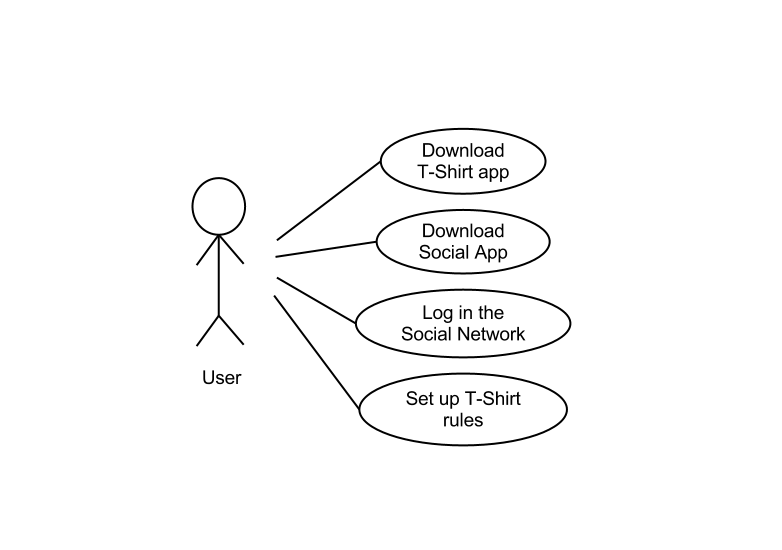
\includegraphics[scale=0.35]{img/architecture-usecase2.png}
\caption{Use case for the second design}
\label{fig:use-case2}
\end{figure}

\begin{figure}[h!]
\centering 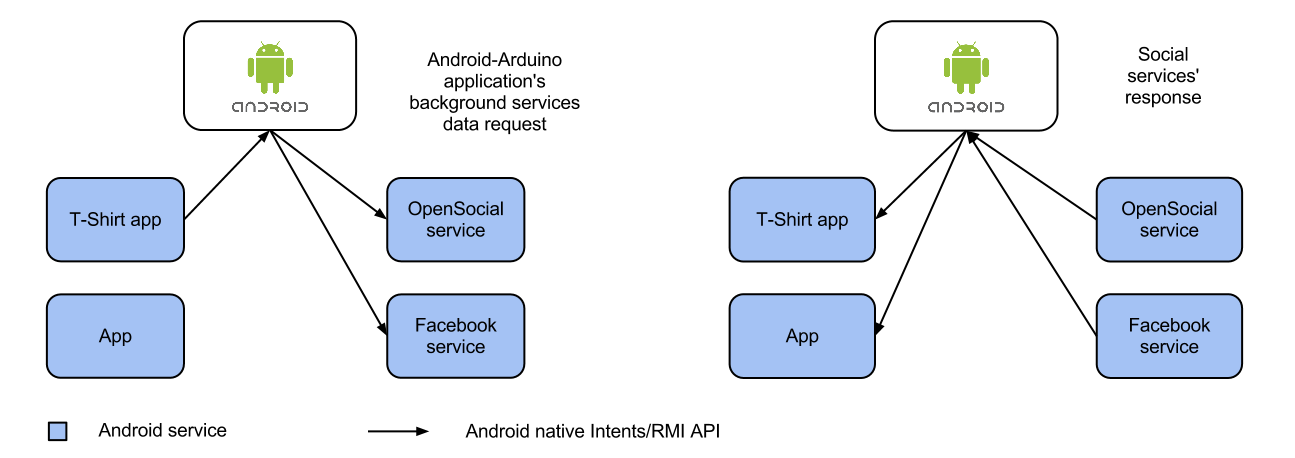
\includegraphics[scale=0.35]{img/architecture-reqresp.png}
\caption{?}
\label{fig:reqresp}
\end{figure}

\newpage
\section{Architecture diagram}

\todo{
	needs to be rewritten
}
The API layer is the social service layer. It uses androids build in broadcast intents to send and
recive data to social services. Included in the social service we have classes that extends Intent
class to indicate if its a social Post, social Group, social Image, social User etc. Multiple apps
can use the API layer to send and retrive this data.

Example:
The API layer is connected with twitter. Twitter retrives a new post and the API layer sends out
a broadcast intent marked as $SOCIAL_POST_IN$. The android OS see who are listeneing to $SOCIAL_POST_IN$ and relay the message to all connected apps. The Developed app now has the post. If the developed app wants to send a post it sends an intent with $SOCIAL_POST_OUT$ that our API can pick up.

The bluetooth protocol in the application is a framework that the developed application includes
to be able to send and recive raw data from the arduino board. It includes handshake and
confirmation commands that is similar to tcp.

The arduino board includes a wrapper around the input/output of the firmware to connect to our protocol.

\section{Sequence Diagram}
The sequence diagram shows off a sample run of connecting and requesting information from a social service etc. the t-shirt application requests friendlist from facebook and age of friend 'Anna'.
\newpage
\begin{figure}[h!]
\centering 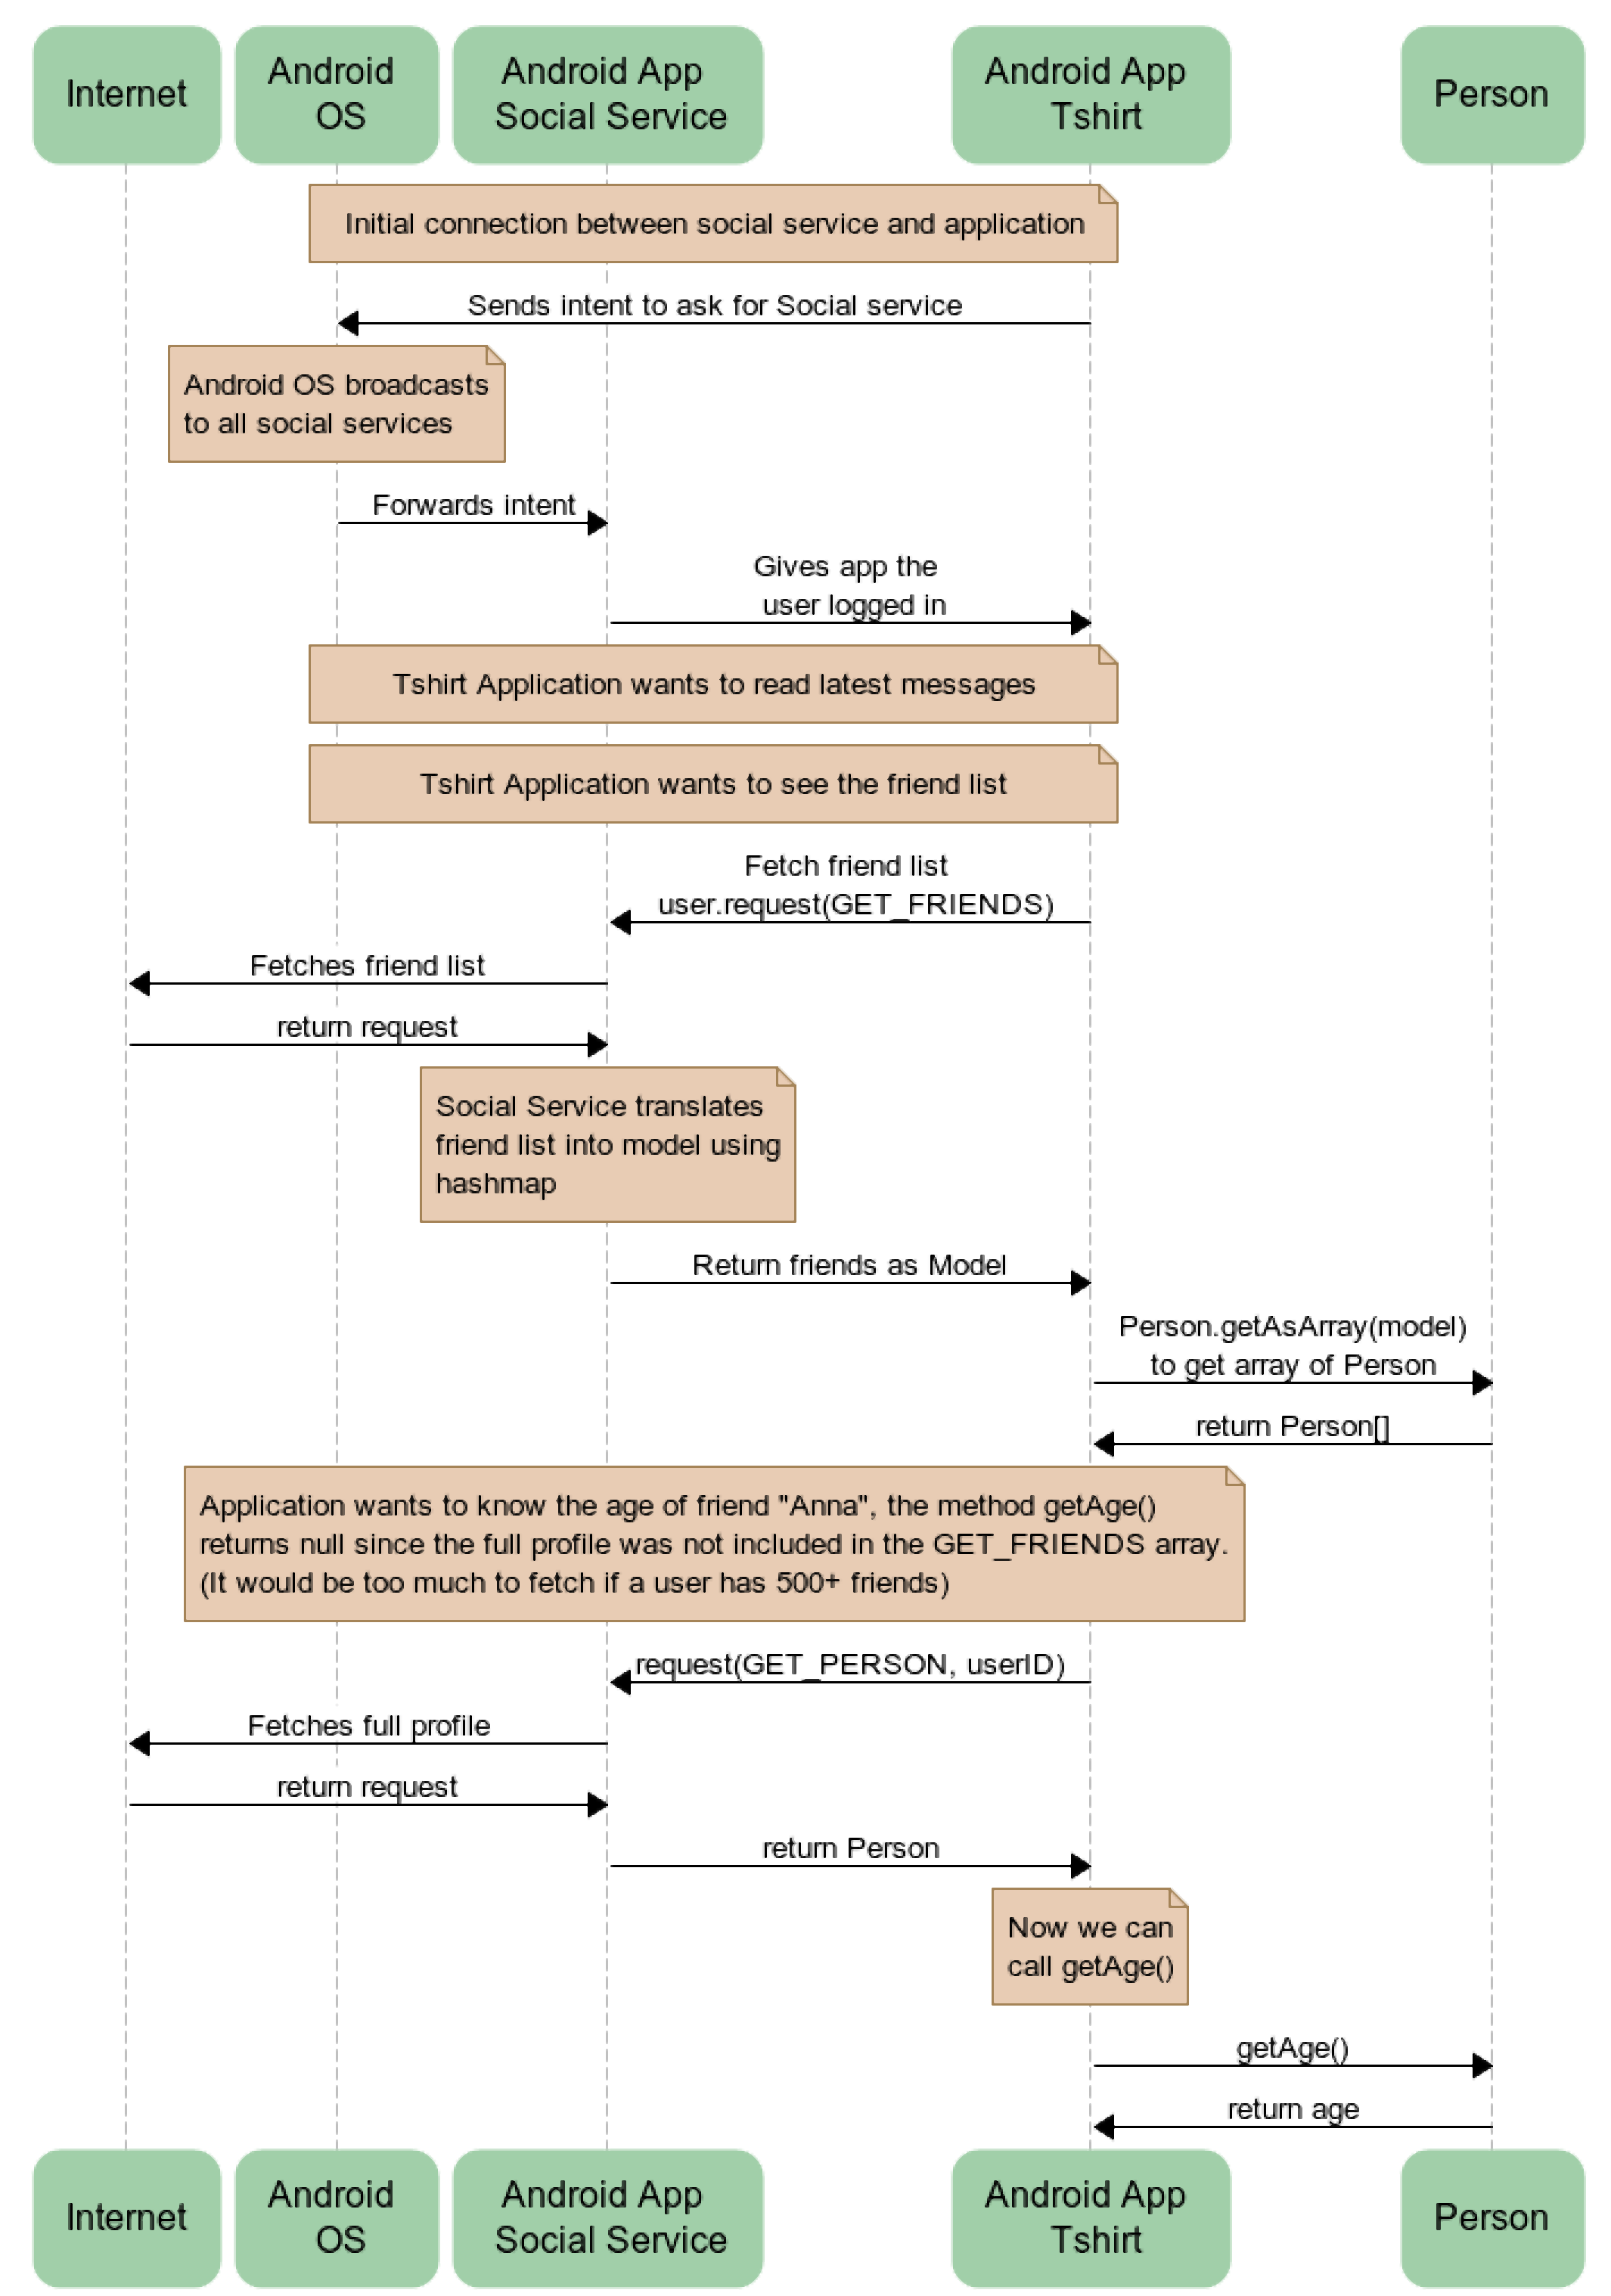
\includegraphics[width=1.0\textwidth]{img/sequenceDiagramSocialService.png} \caption{Sequence Diagram Social Service}
\label{fig:sequenceDiagramSocialService}
\end{figure}

\section{Package Structure}
The system can be divided into smaller sections. This section describes some of the structures
we have divided the system into. The most obvious distinction is between the Java code runs
on the Android platform and the C code which is executed by the Arduino platform.
The Java code is again divided into packaged libraries as described below.

\subsection{Java Code}
\begin{itemize}
\item{no.ntnu.osnap.com}\newline
Communication Library contains every class to establish a connection with a remote device using a general protocol interface. The actual details of the communication such as
Bluetooth, cable, WiFi, stream-based or sockets are hidden away from the user. This is to provide a simple and generic interface to all supported communication methods. The
user can easily add new communication types by extending an abstract class.
\item{no.ntnu.osnap.com.testing}\newline
Test units and sample programs for the ComLib. These are simple test applications that are run on the Android to test if the ComLib is communication correctly using the specified
protocol.
\item{no.ntnu.osnap.social}\newline
Social Library provides an easy to use interface between social networks such as Facebook, Twitter and Myspace and any application or service running on the Android platform.
The SocialLib also provides some general data models such as Person, Group or Post which are concepts that are similar between any social network. 
\item{no.ntnu.osnap.social.testing}  \newline
Test units and sample programs for the SocialLib.
\end{itemize}

\subsection{Arduino C code}
C source code for the Arduino firmware supporting the ComLib protocol.

\section{The ComLib Protocol}

The protocol is a basic set of rules defined for how devices can communicate to the ardunio. Software needed to be implemented on both sides in addition to these rules to be able to use this protocol. The protocol in itself is created by us, and has seen much editing in terms of which instructions was to be included, and how the communication was to be executed. With the current design the arduino cannot initiate the communication, but is instead a passive device. For all instructions sent by any device to the arduino, the arduino sends a response, if only just to acknowledge that it is finished executing the corresponding tasks. If the instruction is asking for information form the arduino, then the response will contain the corresponding information in the "Content" field. An overview of the current instructions in the protocol can be seen in Table~\ref{tbl:opcodes}.

\begin{table}
	\begin{tabular}{ | c | c | p{1.5cm} | p{1.7cm} | p{6cm} |}
		\hline
		\textbf{Name} & \textbf{OPCODE} & \textbf{Flag} & \textbf{Content} & \textbf{Description} \\ \hline
		Ping & 0x00 & N/A & N/A & Pings the arduino, to check that it's there \\ \hline
		Text & 0x01 & N/A & Text to send & Sends text to the arduino, which then displays it depending on the implementation on the ardunio \\ \hline
		Sensor & 0x02 & Sensor number & N/A & Requests sensor information from the arduino \\ \hline
		Pin pulse & 0x03 & Pin number & N/A & Sends a 500ms pulse on the specified pin \\ \hline
		Pin read & 0x04 & Pin number & N/A & Reads the current digital state of the specified pin on the arduino \\ \hline
		Pin write & 0x05 & Pin number & Pin value (0~or1) & Writes a digital state of a pin on the arduino \\ \hline
		Response & 0xFE & Opcode & Response content & A response to a previous instruction, where the flag is the opcode for which it is the response to \\ \hline
		Reset & 0xFF & N/A & N/A & Resets the arduino \\ \hline
	\end{tabular}
	\caption{Overview of the protocol's instructions}
	\label{tbl:opcodes}
\end{table}

\subsection{Arduino implementation}
On the arduino all code related to our protocol is abstracted into a ComputerSerial library. This library is a very basic state machine which processes single bytes received (see Figure~\ref{fig:arduino_states}). The user of this library can register local methods to be called with RPC when the corresponding instruction is called.

The instructions follow strict rules on how they are constructed (see Table~\ref{tbl:instr_struct} for sizes of the different parts). Each instruction has to start with a "start-byte" which is always 0xFF. The next part is the size, which tells the number of bytes to come for this instruction (including the size byte itself). The rest is defined from which instruction is sent, but it is important to remember that the content cannot be empty, and has to at least contain 1 byte. This byte however, is not necessarily read or used.

\begin{table}
	\begin{tabular}{c|c|c|c|c|c|}
		\cline{2-6}
		& \textbf{Start-byte} & \textbf{Size} & \textbf{Opcode} & \textbf{Flag} & \textbf{Content} \\ \hline
		\multicolumn{1}{|c|}{\textbf{Size}} & 1 & 1 & 1 & 1 & 1-252 \\ \hline
	\end{tabular}
	\caption{The byte-structure of instructions}
	\label{tbl:instr_struct}
\end{table}

\begin{figure}
	\centering
	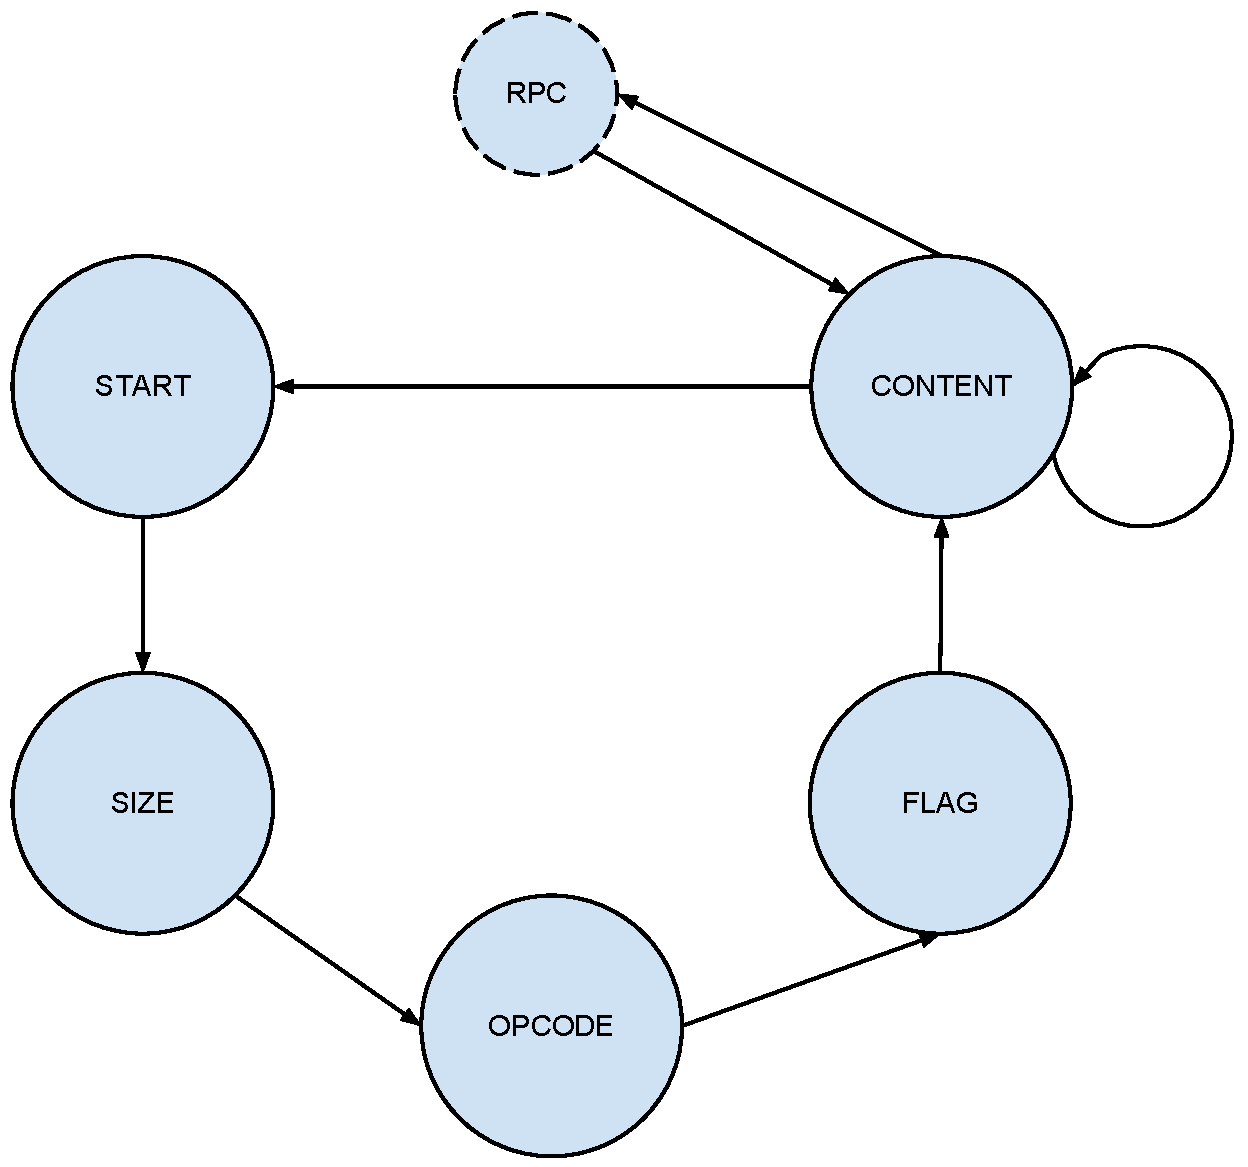
\includegraphics[width=\textwidth, keepaspectratio]{img/arduino_state-machine.pdf}
	\caption{The arduino's state-machine}
	\label{fig:arduino_states}
\end{figure}
